% -*- latex -*-

\documentclass[twocolumn]{article}

\usepackage{amsfonts}
\usepackage{amssymb}
\usepackage{amsmath}
\usepackage{graphicx}
\usepackage{varioref}
\usepackage{fancyvrb}
\usepackage{cite}
\usepackage{xspace}
\usepackage[pdfstartview=FitH]{hyperref}

\title{Divergent Color Maps for Scientific Visualization}

\author{Kenneth~Moreland}

% Commands I use for citing.
\newcommand{\lcite}[1]{~\cite{#1}}
\newcommand{\scite}[1]{~\cite{#1}}

% Avoid putting figures on their own page.
\renewcommand{\textfraction}{0.05}
\renewcommand{\topfraction}{0.95}

% Make sure this is big enough so that only big figures end up on their own
% page but small enough so that if a figure does have to be on its own
% page, it won't push everything to the bottom because it's not big enough
% to have its own page.
\renewcommand{\floatpagefraction}{.75}

\newcommand{\sticky}[1]{\textsc{[#1]}}

\newcommand{\RGB}{RGB\xspace}
\newcommand{\CMYK}{CMYK\xspace}
\newcommand{\XYZ}{XYZ\xspace}
\newcommand{\Lab}{CIELAB\xspace}
\newcommand{\Luv}{CIELUV\xspace}
\newcommand{\Msh}{Msh\xspace}
\newcommand{\DeltaE}{\ensuremath{\Delta{}E}\xspace}

\begin{document}

\maketitle

\begin{abstract}
  One of the most fundamental features of scientific visualization is the
  process of mapping scalar values to colors.  This processes allows us to
  view scalar fields by coloring surfaces and volumes.  Dispite the
  importance of this mapping operation, the majority of scientific
  visualization tools and research are still using a color map that is
  famous for its ineffectiveness: the rainbow color map.  The rainbow color
  map, which na\"{i}vely sweeps through the most saturated colors a display
  can reproduce in the order of the colors in a rainbow, is well known for
  its abilities to obscure data, introduce artifacts, and confuse users.

  Although many other color maps have been proposed and used, none have
  been adopted by the visualization community as a good default in
  scientific visualization.  In this paper we explore the use of divergent
  color maps (sometimes also called bipolar color maps) for use in
  scientific visualization.  We conclude with a divergent color map that
  generally performs well in scientific visualization applications.  This
  color map is a clear replacement for the rainbow color map and can
  hopefully, once and for all, kill the use of the rainbow color map for
  serious scientific visualization applications.
\end{abstract}

\section{Introduction}
\label{sec:Introduction}

At its core, visualization is the process of providing a visual
representation of data.  One of the most fundamental and important aspects
of this process is the mapping of numbers to colors.  This mapping allows
us to pseudocolor an image or object based on varying numerical data.
Obviously, the choice of color map is important to allow the viewer to
easily perform the reverse mapping back to scalar values.

\begin{figure}
  \centering
  
\includegraphics[width=2.5in]{images/RainbowBar}
  \caption{The rainbow color map.  Know thy enemy.}
  \label{fig:RainbowColorMap}
\end{figure}

By far the most common color map used in scientific visualization is the
rainbow color map, shown in Figure~\ref{fig:RainbowColorMap}.  In a recent
review on the use of color maps, Borland and Taylor\scite{Borland07} find
that the rainbow color map was used as the default in 8 out of the 9
toolkits they examined.  Borland and Taylor also find that in IEEE
Visualization papers from 2001 to 2005 the rainbow color map is used 51
percent of the time.

But despite its popularity, the rainbow color map has been shown to be a
poor choice for a color map in almost all problem domains.  This well
studied field of perception shows that the rainbow color map obfuscates,
rather than clarifies, the display of data in a variety of ways.  The
choice of a color map can be a complicated decision that changes based on
the visualization type and problem domain, but the rainbow color map is a
poor choice in almost all of them.

So why are so many visualization scientists and developers, experts who
should know better, still using the rainbow color map?  The answer is
unknown; there are many contributing factors.  Surely two main factors
heavily contribute.  The first is the ease at which the rainbow color map
can be created.  I myself am guilty of creating my first rainbow color map
long before learning anything about color spaces and human perception.  It
was my first choice and I was pleased with the colorful images, ignorant of
their dubious scientific value.

A second major contributor to the dominance of the rainbow color map is the
lack of a clear alternative, especially in terms of scientific
visualization.  There are certainly many publications that recommend some
very good choices for color maps\lcite{Ware04,Brewer05}.  However, each has
its sets of features and detractors, and the choice of the ``right'' one is
difficult.

This paper is a concluding report on the quest for finding a good default
color map for a general purpose scientific visualization application.  The
color map derived here is an all-around good performer: it works well for
low and high frequency data, orders the data, is perceptually linear,
behaves well for observers with color-deficient vision, and has reasonably
low impact on the shading of three dimensional surfaces.


\section{Previous Work}
\label{sec:PreviousWork}

This previous work section is divided into two parts.  The first part is a
quick review on previously proposed color maps and lists the benifits and
detractors of each.  The second section is a quick review on color spaces,
which are used heavily in the subsequent discussions in this paper.

\subsection{Color Maps}
\label{sec:PreviousWork:ColorMaps}

\begin{figure}
  \centering
  
\includegraphics[width=2.5in]{images/GrayscaleBar}
  \caption{The grayscale color map.}
  \label{fig:GrayscaleColorMap}
\end{figure}
Let us start with perhaps the simplest color map of all: the grayscale
color map shown in Figure~\ref{fig:GrayscaleColorMap}.  Completely devoid
of any chromaticity, this map relies entirely on luminance to demonstrate
the numerical value.  Although a very simple map to create and use, this
map is surprisingly effective as the human visual system is most sensitive
to changes in luminance\lcite{Ware04,Mullen85}.  The grayscale color map is
used heavily in the image processing and medical visualization fields.

\begin{figure}
  \centering
  
\includegraphics[width=2.5in]{images/GrayscaleLocality}
  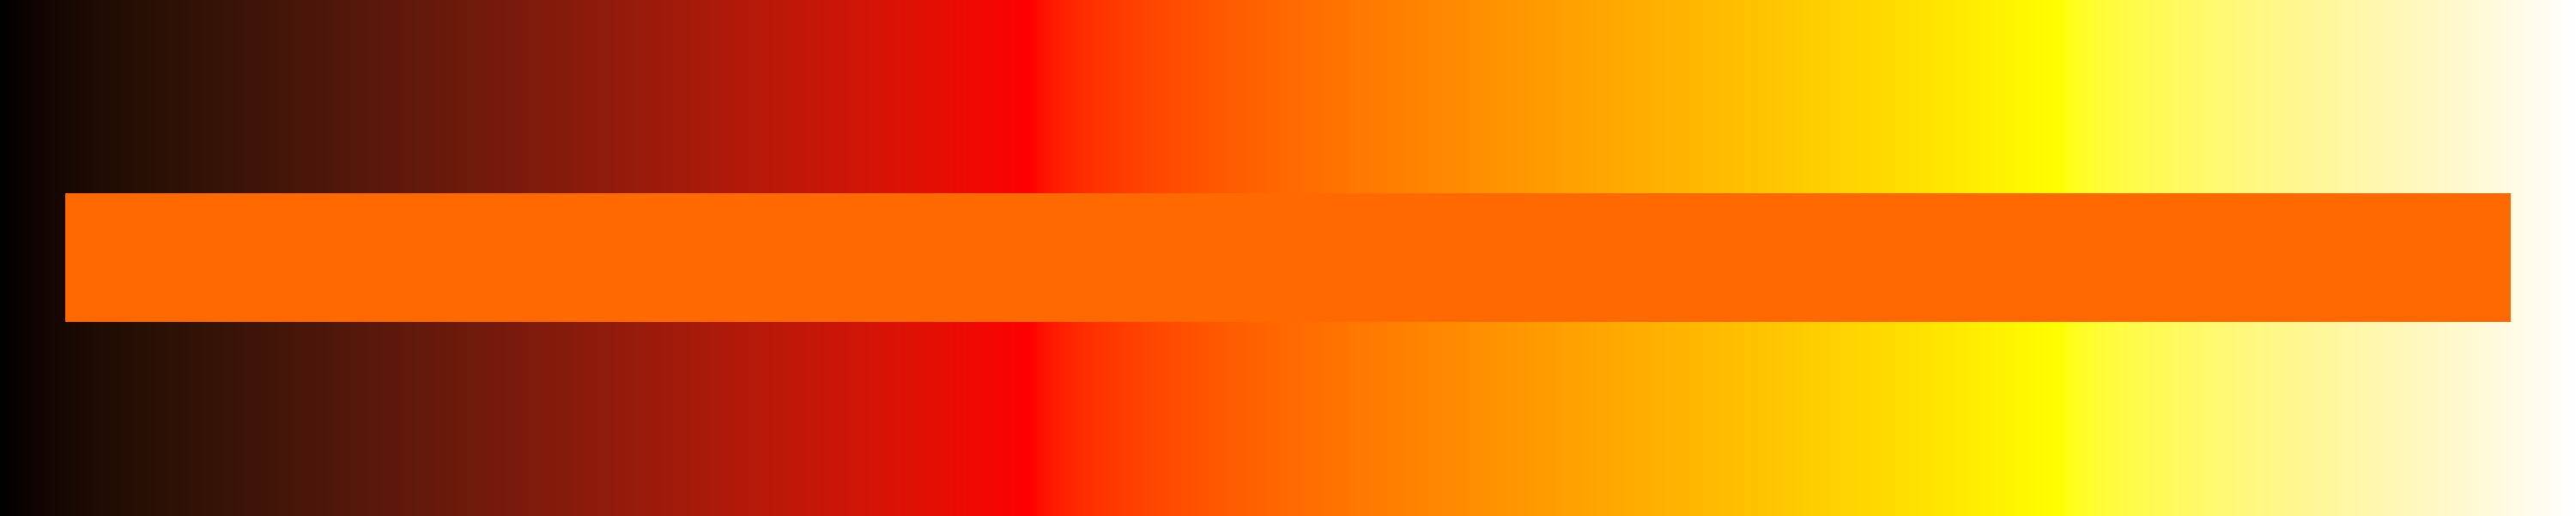
\includegraphics[width=2.5in]{images/BlackBodyLocality}
  \caption{Pixels of the same luminance may look different depending on the
    surrounding pixels (as demonstrated on the top), but color perception
    is relatively stable (as demonstrated on the bottom).}
  \label{fig:GrayscaleLocality}
\end{figure}
The grayscale color map also has a couple of detractors.  One problem is
that a human's perception to brightness is subject to the brightness of the
surrounding area.  Thus, when asked to compare the luminance of two objects
separated by distance and background, human subjects error up to 20\%.
This effect is demonstrated in Figure~\ref{fig:GrayscaleLocality}.  The
problem can be corrected by adding a chromaticity shift.

\begin{figure}
  \centering
  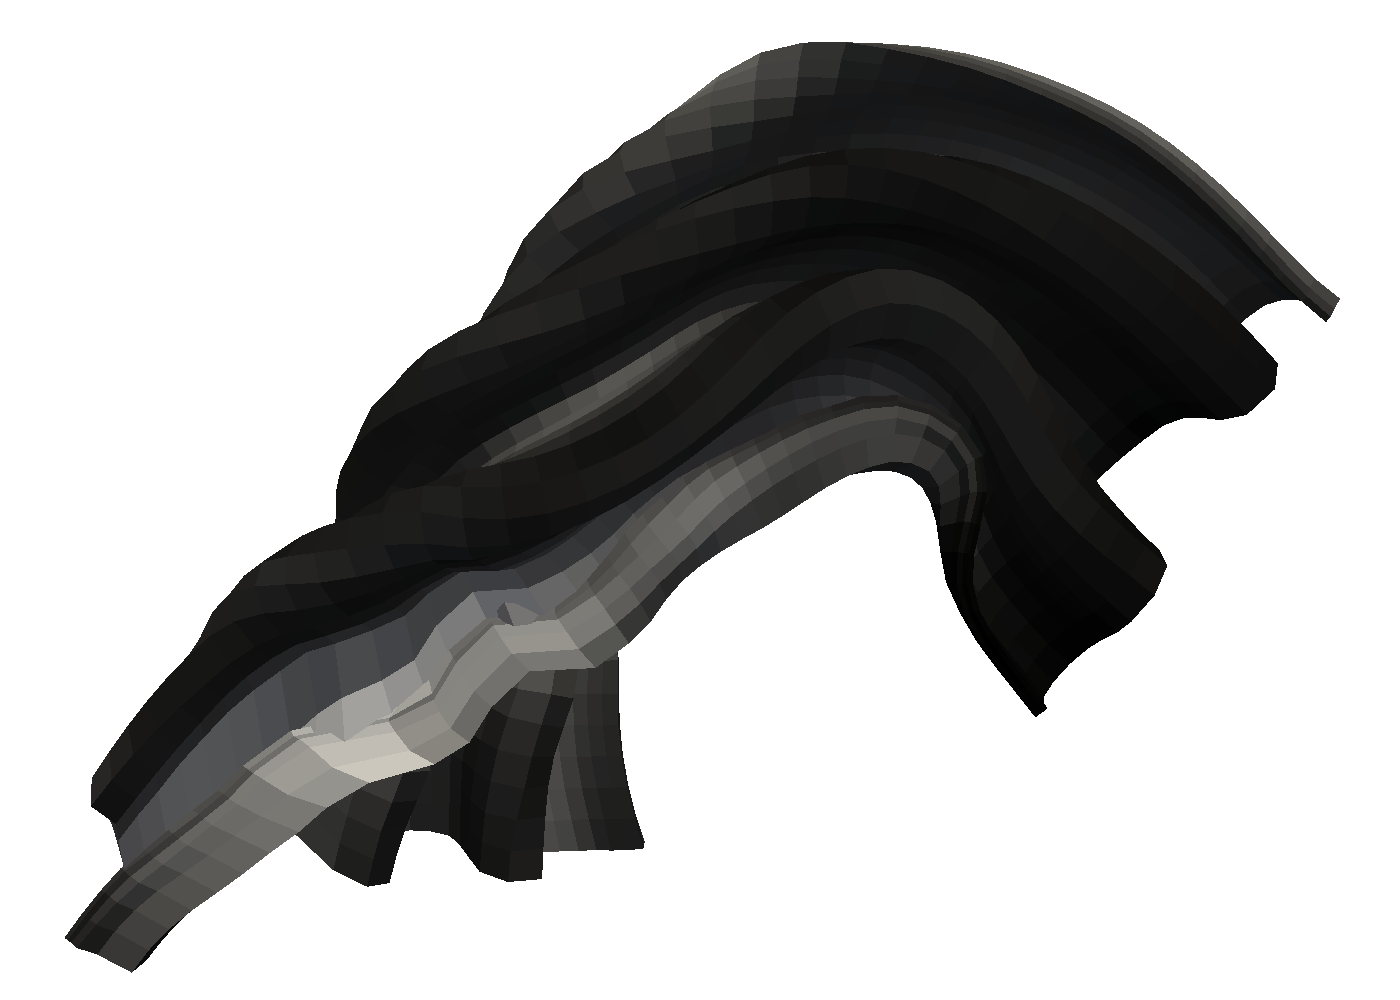
\includegraphics[width=1.25in]{images/GrayscaleShading}
  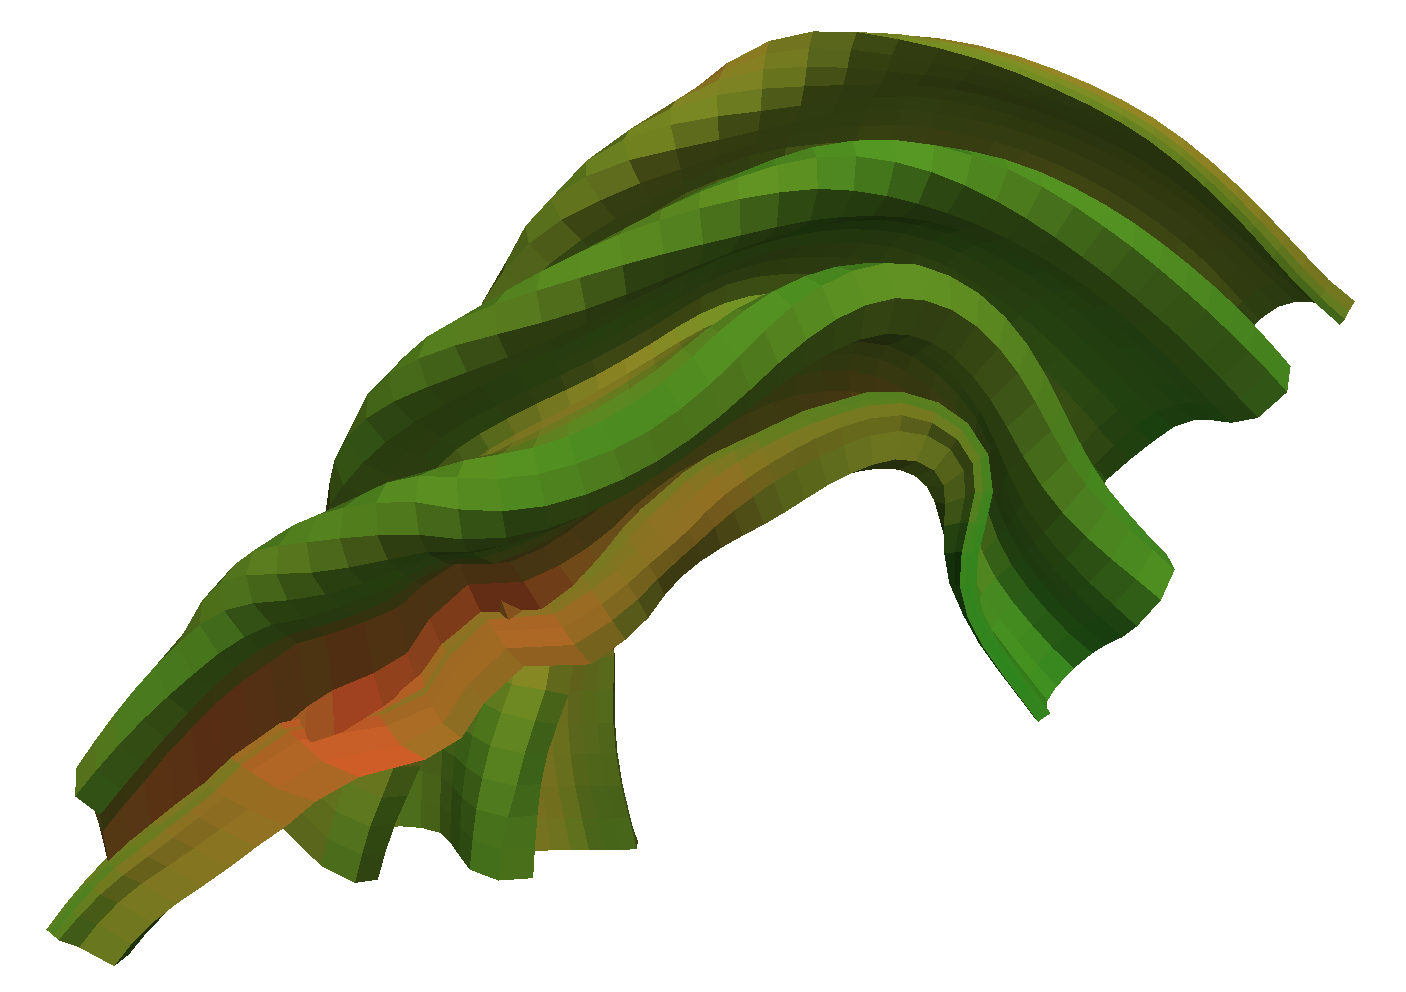
\includegraphics[width=1.25in]{images/IsoluminantShading}
  \caption{Maps with big changes in luminance hides shading cue important
    for determining 3D structure whereas isoluminant maps minimize shading
    interference.}
  \label{fig:LuminanceVsShading}
\end{figure}
Another problem with grayscale color maps that is of greater concern for
general purpose scientific visualization is its interference with surface
shading.  The shading of 3D surfaces based on light sources is of utmost
importance for perceiving the surface shape.  These shading cues are
composed almost entirely of luminance shifts.  Thus the luminance shift of
the grayscale color map mask the surface luminance shifts, especially in
the darker part of the spectrum.  The problem cannot be corrected without a
major reduction in the range the luminance shifts in the color map.

\begin{figure}
  \centering
  
\includegraphics[width=2.5in]{images/Green2RedBar}\qquad
  
\includegraphics[width=2.5in]{images/Cyan2MauveBar}
  \caption{Isoluminant color maps.  The green to red color map is popular
    because it uses a pair of opponent colors, but the cyan to mauve color
    map is much easier to see by individuals with deuteranope or protanopic
    vision.}
  \label{fig:IsoluminantColorMap}
\end{figure}
Another class of color maps that is often suggested for use with 3D
surfaces is the isoluminant color map that is demonstrated in
Figure~\ref{fig:IsoluminantColorMap}.  Somewhat opposite to the grayscale
map, an isoluminant map maintains a constant (perceptual) luminance and
relies entirely on chromatic shifts.  An isoluminant color map is
theoretically ideal for mapping onto shaded surfaces, as is demonstrated in
Figure~\ref{fig:LuminanceVsShading}.

Isoluminant color maps are not without their detractors, however.  Human
perception is less sensitive to changes in saturation or hue than changes
in luminance, especially for high frequency data\lcite{Rogowitz96}.
Holding the luminance constant also restricts the colors that can be
represented.  Thus, the isoluminant color map will have a lower fidelity
than one in which the luminance is allowed to change.  Isoluminant color
maps also tend to look dull and ugly, which means that a casual user will
almost never choose one over a more vibrant color map like, say, the
rainbow color map.

However, as vibrant as the rainbow color map might be, it is actually an
extremely poor choice.  Based on the colors of light at different
wavelengths, the rainbow color map's design has nothing to do with how
humans perceive color.  This results in multiple problems when humans try
to do the reverse mapping from colors back to numbers.

The first problem with the rainbow color map is that it is sensitive to
deficiencies in vision.  A significant proportion of the population, most
of which are males, cannot distinguish between the red and green colors.
These unfortunate soles cannot distinguish many colors considered ``far
appart'' in the rainbow color map\lcite{Light04}.

The second problem is that the colors do not follow any natural perceived
ordering.  Perceptual experiments show that although a test subject, with
no prior training, will always order grayscale colors in order of luminance,
the test subjects will order rainbow colors in numerous different
ways\lcite{Ware04}.

\begin{figure}
  \centering
  
\includegraphics[width=1.0in]{images/GrayscaleSpatialContrast}
  \qquad
  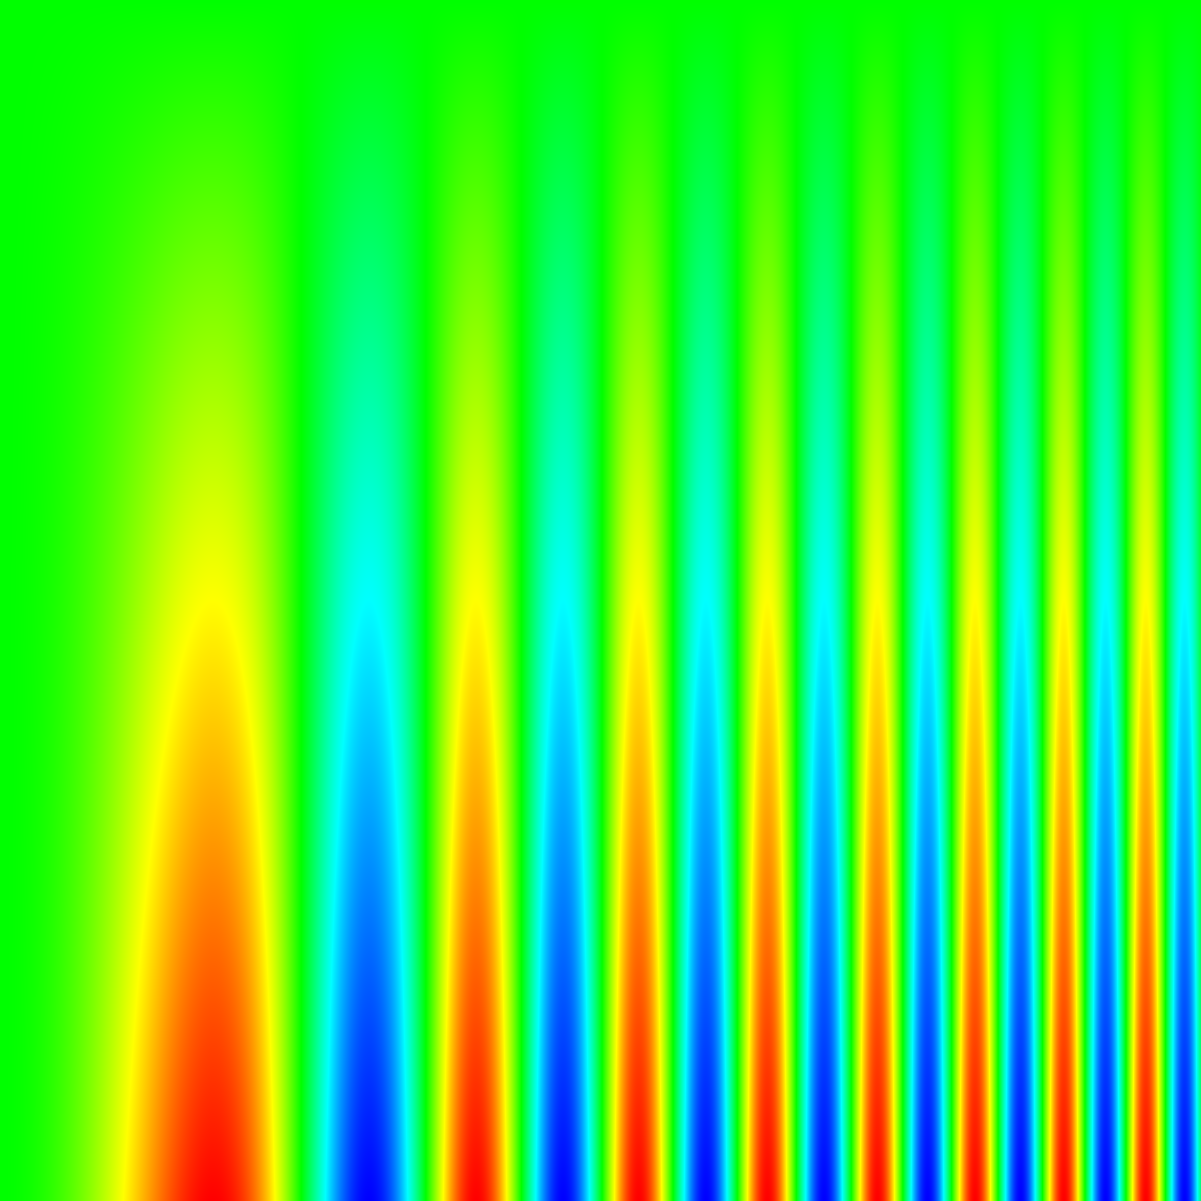
\includegraphics[width=1.0in]{images/RainbowSpatialContrast}
  \caption{A spatial contrast sensitivity function.  The frequency of the
    function increases from left to right, and the contrast increases from
    top to bottom.  Notice that the grayscale mapping faithfully reproduces
    the function.  The rainbow color mapping hides the variation in the low
    contrast region and appears less smooth in the high-contrast,
    low-frequency region.}
  \label{fig:RainbowSpatialContrast}
\end{figure}

A third problem is that the perceptual changes in the colors are not
uniform.  The colors appear to change faster in the cyan and yellow
regions, which can cause Mach bands in those regions.  The colors appear to
change slower in the blue, green, and red regions, which creates larger
bands of color.  Within these bands it can hide important changes in the
underlying data.  Thus, the nonuniform perceptual changes works to
simultaneously introduce artifacts and obfuscate real
data\lcite{Borland07} as demonstrated in
Figure~\ref{fig:RainbowSpatialContrast}.

These color maps comprise the most commonly used in literature and tools
today.  Other color maps are proposed by Ware\scite{Ware04} as well as
several others.  Most are similar in spirit to those here with uniform
changes in luminance, saturation, or hue or some combination thereof.

\subsection{Color Spaces}
\label{sec:PreviousWork:ColorSpaces}

The remainder of this paper relies on using different color spaces to
describe color map generation.  This section quickly reviews some of these
color spaces.

All color spaces are based on the tri-color stimulus theory, which states
that any perceived color can be uniquely represented by a 3-tuple
\sticky{Reference}.  This result is a side effect of the fact that there
are exactly 3 different types of color receptors in the human eye.

The color space most frequently used is the \RGB color space
\sticky{Reference}.  This color space is adopted by many graphics packages
such as OpenGL and is presented to users by just about every computer
application in existence that provides a color chooser.  The three values
in the \RGB color space refer to the intensity output by each of the three
wavelengths of light used by monitors, televisions, and projectors to
create colors.  There is also a similar \CMYK color space that defines
colors by how printers mix ink \sticky{Reference}.

Although the \RGB and \CMYK color spaces are good for many practical
purposes, since they are defined exactly over the gamut of colors that can
be displayed, it is sometimes useful to define colors over the gamut of
visible colors.  However, it is not as useful for describing colors that
are visible but not representable by the display.  To this end the
International Commission on Illumination (better known as CIE from its
French title, the \emph{Commission Internationale de l'\'{E}clairage})
convened in 1931 and defined the \XYZ color space \sticky{Reference}.  The
\XYZ color space provides a convenient way to consistently describe all
visible colors without being tied to any particular display device.

The \XYZ color space, however, is still defined by the physical properties
of light.  Movements within the \XYZ space are not perceptually linear.  To
address the need for a perceptually linear color space, the CIE developed
two more color spaces in 1976: \Lab and \Luv.  The choice between the two
is fairly arbitrary; this paper uses \Lab \sticky{Reference}.

\Lab is an approximation of how humans perceive light.  The Euclidean
distance between two points is the approximate perceived difference between
the two colors.  This Euclidean distance in \Lab space is known as \DeltaE
and makes a good metric for comparing color differences
\sticky{Reference?}.


\section{Color Map Requirements}
\label{sec:ColorMapRequirements}

Our ultimate goal is to design a color map that works well for in
general-purpose scientific visualization.  It should work well for a wide
breadth of tasks and users.  As such we have the following requirements.

\begin{itemize}
\item The map yields images that are colorful and vibrant.
\item The perceptual interpolation matches the underlying scalars the map
  represents.
\item The map maximizes the perceptual resolution.
\item Interference the shading of 3D surfaces is minimal.
\item The map is not sensitive with vision deficiencies.
\item The order of the colors should be natural.
\end{itemize}

The reasoning behind most of these requirements is self explanatory.  The
requirement that the color map be ``pretty,'' however, is not one often
found in the scientific literature.  After all, the attractiveness of the
color map, which is difficult to quantify in the first place, has little to
do its effectiveness in conveying information.  Nevertheless, aesthetic
appeal is important as users will use that as a criteria in selecting
visualization products and generating images.

% \begin{itemize}
% \item Due to the proliferation of visualization programs and images using
%   the rainbow color map, many users will have ``learned'' the order of the
%   colors and will continue to have to use them.  Our color map should try
%   not to break that convention.
% \end{itemize}

Several of these requirements are contradictory, which makes choosing a
general purpose color map so difficult.  All of the examples in
Section~\ref{sec:PreviousWork:ColorMaps} excel in some of the requirements,
but fail completely in one or more of the others.  It is impossible to have
a color map that performs perfectly in all of the requirements.  Our color
map must be a compromise that works reasonable well in all areas.

\section{Acknowledgements}

This work was done at Sandia National Laboratories.  Sandia is a
multiprogram laboratory operated by Sandia Corporation, a Lockheed Martin
Company, for the United States Department of Energy's National Nuclear
Security Administration under contract DE-AC04-94AL85000.

\bibliographystyle{plain}
\bibliography{ColorMaps}

\end{document}
